\chapter{Methodology}

\section{Data generation}

  Observations $x \in \mathbb{R}^n$ are drawn from a uniform distribution,
  while each latent coefficient vector $\beta_j \in \mathbb{R}^n$
  is drawn from a multivariate Gaussian distribution.
  Each vector $\beta_j$ is a column of the coefficient
  matrix $\beta \in \mathbb{R}^{n \times m}$ and fixed beforehand.
  Instead of choosing arbitrary mean vector and covariance
  matrix as parameters of the multivariate Gaussian distribution,
  these parameters are drawn at random. Also, the covariance matrix
  should be positive semi-definite. Therefore, a normal-Wishart
  is used to generate a random mean vector and a precision matrix.
  The final covariance matrix is obtained by inverting the sampled
  precision matrix.

  \begin{figure}[ht]
    \begin{center}
      \resizebox{.85\textwidth}{!}{
        \begin{tikzpicture}


  % Explained variables
  \node[latent] (y) {$y$};

  % Gaussian noise
  \node[latent, above=1.5 of y, xshift=-4.5cm] (w) {$w$};
  \node[const, above=0.5 of w] (noisemu) {};
  \node[const, above=0.5 of w]  (noisesigma) {};
  \factor[above=of w] {w-f} {above:$w \sim \mathcal{N}(0, 1)$} {noisemu, noisesigma} {w};

  % Observations
  \node[obs, above=1.5 of y, xshift=-2.5cm] (x) {$x$};
  \node[const, above=0.5 of x] (xlb) {};
  \node[const, above=0.5 of x]  (xub) {};
  \factor[above=of x] {x-f} {above:$x \sim \mathcal{U}(0, 1)$} {xlb, xub} {x};

  % Coefficients
  \node[latent, above=1.5 of y, xshift=2.5cm] (beta) {$\beta$};

  % Connect x and w to y
  \edge[-] {beta} {y};
  \edge[-] {x} {y};
  \edge[-] {w} {y};

  % Mean vector and precision matrix
  \node[latent, above=3.3 of beta, xshift=1.5cm]  (Lambda)        {$\Lambda$};
  \node[latent, above=1.5 of beta, xshift=-1.5cm] (mu)        {$\mu$};
  \factor[above=of beta] {beta-f} {right:$\beta_j \sim \mathcal{N}(\mu, \Lambda^{-1})$} {mu, Lambda} {beta};

  % Hyper-parameters of mu
  \node[const, above=1.4 of mu, xshift=-1.6cm] (lambda0) {$\lambda_0$};
  \node[const, above=1.4 of mu, xshift=0.0cm] (mu0) {$\mu_0$};
  \factor[above=of mu] {mu-f} {left:$\mu \sim \mathcal{N}(\mu_0, (\lambda_0 \Lambda)^{-1})$} {lambda0, mu0, Lambda} {mu};

  % Hyper-parameters of Lambda
  \node[const, above=1.0 of Lambda, xshift=-0.8cm] (nu0) {$\nu_0$};
  \node[const, above=1.0 of Lambda, xshift=0.8cm] (W0) {$W_0$};
  \factor[above=of Lambda] {W-f} {left:$\Lambda \sim \mathcal{W}(W_0, \nu_0)$} {W0, nu0} {Lambda};
  
  % Time Plate
  \plate[xshift=0.1cm, yshift=0.0cm] {plate-t} { (w)(w-f)(x)(x-f)(y) } {$t$};
  
  % Output Plate
  \plate[yshift=0.4cm] {plate-j}{ (y)(beta)(beta-f) } {$j$};

\end{tikzpicture}
      }
    \end{center}
    \caption{Bayesian network representing the randomly generated samples.
        Plate notation indicates variable repetition across time and
        output variables, respectively.}
    \label{bayesnet}
  \end{figure}

  As can be observed from the plate notation in figure \ref{bayesnet},
  coefficient vectors $\beta_j$ are computed only once for each $j$,
  and $w$, $x$, $y$ are sampled at each time step $t$, where $y_j = \beta_j x$.
  Mean vector $\mu$ and precision matrix $\Lambda$ are sampled only once
  from a normal-Wishart distribution.
  Default parameter matrix $W_0$ is the diagonal matrix, prior mean vector $\mu_0$
  is the zero vector, chosen scaling parameter is $1$, and $\nu_0$ has been
  arbitrarily set to $15$.


\section{Recursive Least Squares (RLS) with forgetting factor}

In the standard RLS implementation with forgetting factor,
the weights $\beta$ are estimated incrementally using the following formulas:

\begin{align}
\begin{cases}
    V^{(t)} & = \frac{1}{\nu} \Bigg( V^{(t-1)} - \frac{V^{(t-1)} x_t^T x_t V^{(t-1)}}{1 + x_t V^{(t-1)} (x_t^T} \Bigg) \\
    \alpha^{(t)} & = V^{(t)} x_t^T \\
    e^{(t)} & = y^{(t)} - x_t \hat{\beta}^{(t-1)} \\
    \hat{\beta}^{(t)} & = \hat{\beta}^{(t-1)} + \alpha^{(t)} e^{(t)}
\end{cases}
\end{align}

where $V^{(t)}$ is a matrix of shape $n \times n$, $n$ is the number of explanatory variables
and $e^{(t)}$ is the prediction error on the example retrieved from the Kafka consumer at time step $t$.
In this project, the learning algorithm should be able to handle multiple output variables.
Therefore, such formulation has to be extended to a multi-output case.

\subsection{First approach -- Fully-vectorized version}

This approach is used when the number of output/explained variables is low,
and relies on NumPy's efficient implementation of the dot-product.
Let $B \in \mathbb{R}^{n \times m}$ denote a matrix this time.
Each machine on the cluster computes \textbf{the whole coefficient matrix} $B$
with a different forgetting factor.

\begin{align}
\begin{cases}
    \alpha_t & = V^{(t)} x_t^T \\
    e^{(t)} & = y^{(t)} - x_t \hat{B}^{(t-1)} \\
    \hat{B}^{(t)} & = \hat{B}^{(t-1)} + \alpha_t^T e^{(t)}
\end{cases}
\end{align}

$e^{(t)} \in \mathbb{R}^m$ is vector and $e_j^{(t)}$ is the prediction error
on the output variable $y_j$ retrieved at time $t$ from the Kafka consumer.


\subsection{Second approach -- Distributed version}

The scalability of the algorithm w.r.t. to the number of output variables
is enabled by this second approach. However, it is actually interesting
when the number of output variables is larger than the number of input
variables. At this condition only, the bottleneck of the algorithm
is the computation of $\hat{B}^{(t)}$ and not $V^{(t)}$.
Therefore, such approach is used only when the number of output variables
is sufficiently high. For demonstration purposes, the second approach
is used in the notebook since the number of output variables has been
set to $8$ and the threshold to $6$. Note that this threshold is arbitrary
and is a user preference. In practice, I believe that a reasonable design choice
would be to set the threshold to the vector size from which NumPy starts having
recourse to multithreading.

\begin{align}
\begin{cases}
    \alpha_t & = V^{(t)} x_t^T \\
    e^{(t)} & = y_j^{(t)} - x_t \hat{B}_{\cdot j}^{(t-1)} \\
    \hat{B}_{\cdot j}^{(t)} & = \hat{B}_{\cdot j}^{(t-1)} + \alpha_t^T e^{(t)}
\end{cases}
\end{align}

In the present approach, each machine of the cluster computes one column
of the coefficient matrix $B$. Therefore, each node is assigned an output
variable $j$ and re-estimates $\hat{B}_{\cdot j}^{(t)}$ at each time step $t$.
Also, $e^{(t)}$ is a scalar and represents the prediction error on $y_j$ at time step $t$.


\section{Architecture and Spark implementation}

\begin{figure}[H]
    \begin{center}
        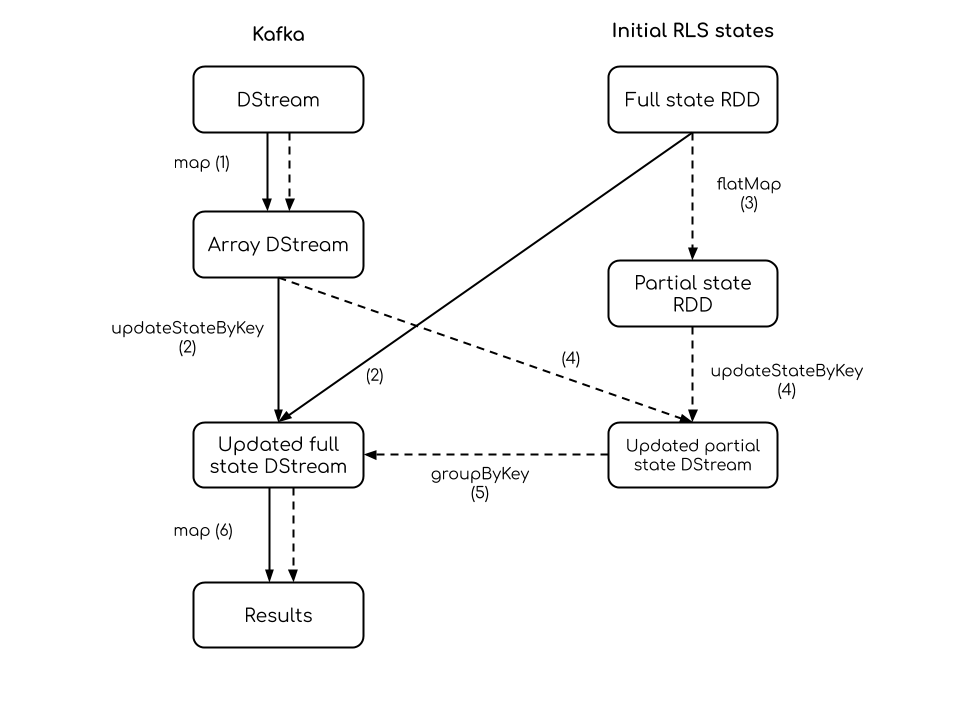
\includegraphics[width=\textwidth, keepaspectratio]{imgs/lineage-graph.png}
        \caption{Lineage graph for the proposed architecture. Dashed lines indicate
            the Spark transformations applied in the distributed version
            and plain lines indicate the transformations applied in the fully-vectorized version.}
        \label{architecture}
    \end{center}
\end{figure}

